\documentclass[../../doc.tex]{subfiles}
\graphicspath{{\subfix{../../img}}}
\begin{document}
    \subsection{Обход препятствия}
    
    Учёт фазовых ограничений в интегральной части функционала качест\-ва~$J$, представленный в работе,
    позволяет лишь приближенно описать условия вида
    $$
        g_i(x) \leqslant 0,
    $$
    которые возникают естественным образом в задаче обхода препятствия.
    Для этого фазовое условие $q$ выбирается таким образом, чтобы штрафовать за приближение траектории к препятствию.

    \begin{remark}
        Для формального решения задачи с подобными условиями,
        необходимо пользоваться методами расширенного лангранжиана~\cite{birgin2009},
        которые предполагают решение серии задач типа~\eqref{eq:discrete-system}-\eqref{eq:discrete-cost}.
        Это приводит к ухудшению асимптотики алгоритмов и тем самым существенному увеличению времени работы программного решения.
    \end{remark}

    Пусть задано некоторое точечное препятствие с центром $e^{\textnormal{obstacle}}$ и радиусом $r_{\textnormal{obstacle}}$.
    Тогда зададим интегральное условие в виде:
    \begin{equation}\label{eq:obstacle-phase}
        q(x) = \left( \left\| e^3(x) - e^{\textnormal{obstacle}} \right\|^2 - r_{\textnormal{obstacle}} \right)^{-2}.
    \end{equation}

    Рис.~\ref{fig:obstacle-task} и Рис.~\ref{fig:obstacle-less-task} демонстрируют траекторию руки при построенном управлении, а также траектории схвата при управлениях, полученных на различных итерациях алгоритма
    для решения задачи целевого состояния~\eqref{eq:ilqr-algo:cost} с фазовым ограничением~\eqref{eq:obstacle-phase} при различных весах на фазовое условие.

    \begin{figure}[ht]
        \begin{center}
            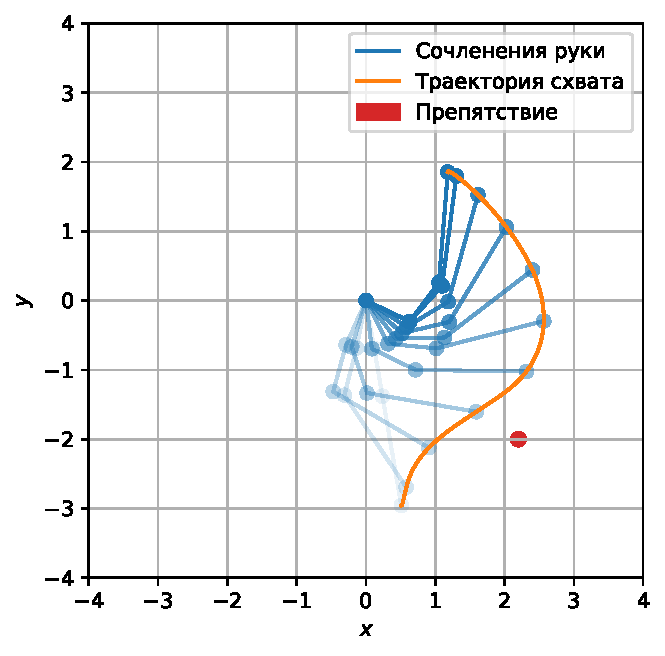
\includegraphics[width=0.49\textwidth]{examples/obstacle_pendulum}
            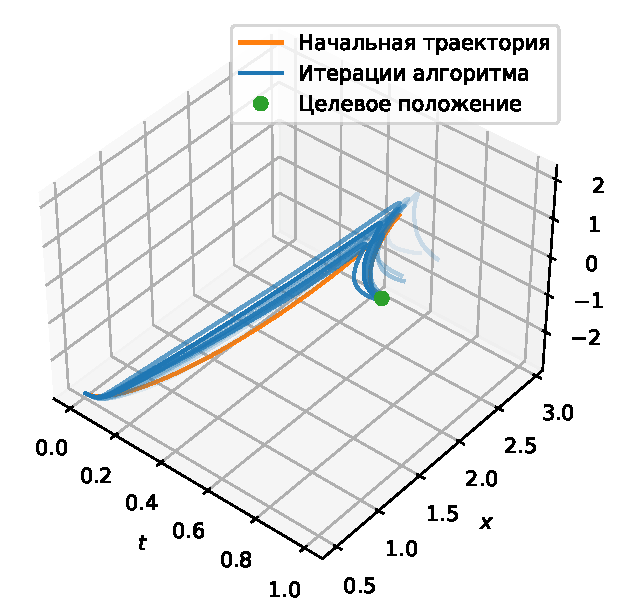
\includegraphics[width=0.49\textwidth]{examples/obstacle_endpoint}
        \end{center}
        \caption{
            Траектория системы при оптимальном управлении и итеративные траектории схвата для задачи обхода препятствия.
            Вес фазового условия $w_1 = 10^{-1}$.
            Алгоритм сошёлся на 10 итерации.
        }
        \label{fig:obstacle-task}
    \end{figure}
    \begin{figure}[t]
        \begin{center}
            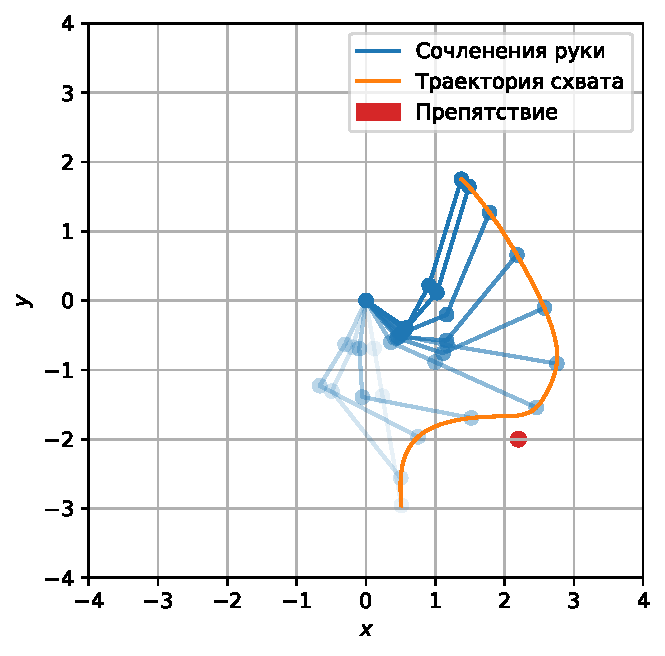
\includegraphics[width=0.49\textwidth]{examples/obstacle_pendulum_less}
            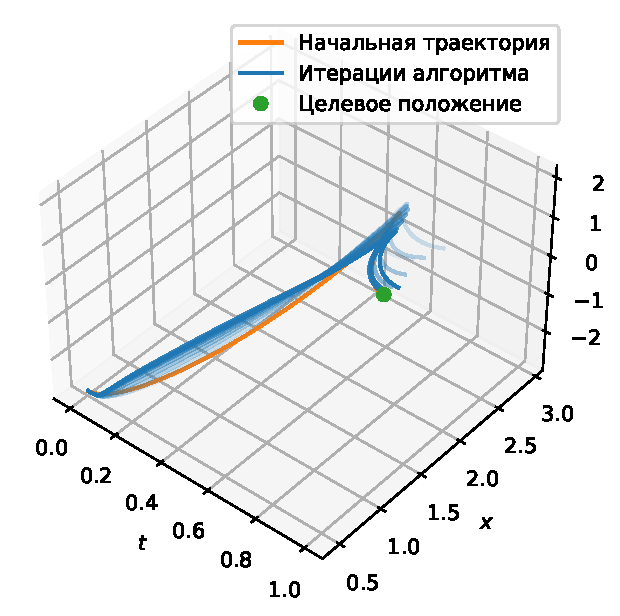
\includegraphics[width=0.49\textwidth]{examples/obstacle_endpoint_less}
        \end{center}
        \caption{
            Траектория системы при оптимальном управлении и итеративные траектории схвата для задачи обхода препятствия.
            Вес фазового условия $w_1 = 2 \cdot 10^{-2}$.
            Алгоритм сошёлся на 8 итерации.
        }
        \label{fig:obstacle-less-task}
        \vspace*{7in}
    \end{figure}

    \ifSubfilesClassLoaded{
        \nocite{*}
        \clearpage
        \bibliographystyle{plain}
        \bibliography{../../refs}
    }{}
\end{document}